\documentclass[]{article}

\usepackage{listings}
\usepackage{float}
\usepackage[a4paper, margin=2cm]{geometry}
\usepackage{dirtytalk}
\usepackage[x11names, svgnames, rgb]{xcolor}
\usepackage[utf8]{inputenc}
\usepackage{tikz}
\usetikzlibrary{snakes,arrows,shapes}
\usepackage{amsmath}

\definecolor{codegreen}{rgb}{0,0.6,0}
\definecolor{codegray}{rgb}{0.5,0.5,0.5}
\definecolor{codepurple}{rgb}{0.58,0,0.82}
\definecolor{backcolour}{rgb}{0.95,0.95,0.92}

\lstdefinestyle{code}{
    backgroundcolor=\color{backcolour},   
    commentstyle=\color{codegreen},
    keywordstyle=\color{blue},
    numberstyle=\tiny\color{codegray},
    stringstyle=\color{codepurple},
    basicstyle=\ttfamily\footnotesize,
    breakatwhitespace=false,         
    breaklines=true,                 
    captionpos=b,                    
    keepspaces=true,                 
    numbers=left,                    
    numbersep=5pt,                  
    showspaces=false,                
    showstringspaces=false,
    showtabs=false,                  
    tabsize=2
}

\definecolor{delim}{rgb}{0.5,0.5,0}
\definecolor{punct}{rgb}{0,0,0.5}
\definecolor{numb}{rgb}{0,0.5,0.5}

\lstdefinelanguage{json}{
    basicstyle=\normalfont\ttfamily,
    numbers=left,
    numberstyle=\scriptsize,
    stepnumber=1,
    numbersep=8pt,
    showstringspaces=false,
    breaklines=true,
    frame=lines,
    backgroundcolor=\color{backcolour},
    literate=
     *{0}{{{\color{numb}0}}}{1}
      {1}{{{\color{numb}1}}}{1}
      {2}{{{\color{numb}2}}}{1}
      {3}{{{\color{numb}3}}}{1}
      {4}{{{\color{numb}4}}}{1}
      {5}{{{\color{numb}5}}}{1}
      {6}{{{\color{numb}6}}}{1}
      {7}{{{\color{numb}7}}}{1}
      {8}{{{\color{numb}8}}}{1}
      {9}{{{\color{numb}9}}}{1}
      {:}{{{\color{punct}{:}}}}{1}
      {,}{{{\color{punct}{,}}}}{1}
      {\{}{{{\color{delim}{\{}}}}{1}
      {\}}{{{\color{delim}{\}}}}}{1}
      {[}{{{\color{delim}{[}}}}{1}
      {]}{{{\color{delim}{]}}}}{1},
}

\lstset{style=code}

\title{RISC-V approach proposal}
\author{Abdelsalam ElTamawy}


\begin{document}

The other possible idea is to instead of construct the graph structure around the module, we can construct the graph structure around the instructions.
Opposite to the other idea, I think this might make things easier when making inter module optimizations but make writing the internals of the modules a bit more difficult.
I think this approach can prove to be more flexible.

The graph will describe directed edges for each wire.

If we take the ADD instruction as an example, what we will be after is representing this graph.

\begin{figure}[H]
	\centering
	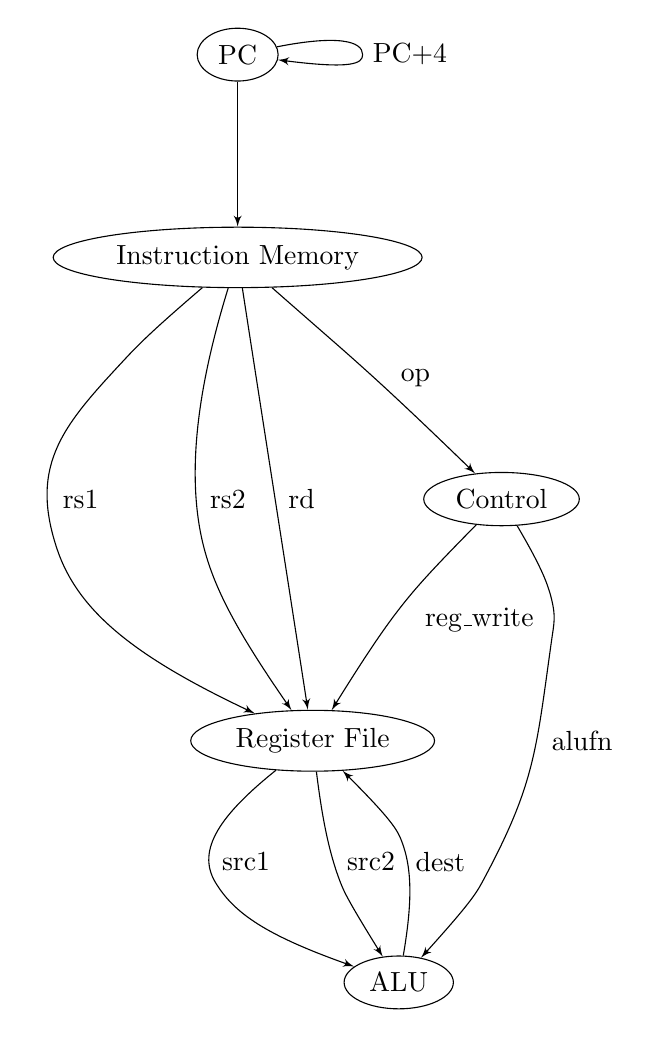
\begin{tikzpicture}[>=latex',line join=bevel,]
		%%
		\node (pc) at (81.243bp,352.0bp) [draw,ellipse] {PC};
		  \node (im) at (81.243bp,279.0bp) [draw,ellipse] {Instruction Memory};
		  \node (reg) at (108.24bp,105.0bp) [draw,ellipse] {Register File};
		  \node (alu) at (139.24bp,18.0bp) [draw,ellipse] {ALU};
		  \node (ctrl) at (176.24bp,192.0bp) [draw,ellipse] {Control};
		  \draw [->] (pc) ..controls (117.27bp,359.15bp) and (126.24bp,356.92bp)  .. (126.24bp,352.0bp) .. controls (126.24bp,348.77bp) and (122.38bp,346.7bp)  .. (pc);
		  \definecolor{strokecol}{rgb}{0.0,0.0,0.0};
		  \pgfsetstrokecolor{strokecol}
		  \draw (143.24bp,352.0bp) node {PC+4};
		  \draw [->] (pc) ..controls (81.243bp,325.79bp) and (81.243bp,316.05bp)  .. (im);
		  \draw [->] (reg) ..controls (75.278bp,78.513bp) and (66.142bp,65.803bp)  .. (73.243bp,54.0bp) .. controls (80.048bp,42.688bp) and (91.876bp,34.838bp)  .. (alu);
		  \draw (84.243bp,61.5bp) node {src1};
		  \draw [->] (reg) ..controls (111.66bp,77.069bp) and (114.16bp,64.569bp)  .. (118.24bp,54.0bp) .. controls (119.6bp,50.489bp) and (121.3bp,46.927bp)  .. (alu);
		  \draw (129.24bp,61.5bp) node {src2};
		  \draw [->] (alu) ..controls (144.01bp,46.14bp) and (144.26bp,58.64bp)  .. (140.24bp,69.0bp) .. controls (138.7bp,72.972bp) and (136.47bp,76.768bp)  .. (reg);
		  \draw (154.24bp,61.5bp) node {dest};
		  \draw [->] (ctrl) ..controls (154.21bp,169.61bp) and (147.7bp,162.7bp)  .. (142.24bp,156.0bp) .. controls (135.91bp,148.23bp) and (129.57bp,139.31bp)  .. (reg);
		  \draw (168.24bp,148.5bp) node {reg\_write};
		  \draw [->] (ctrl) ..controls (189.78bp,168.89bp) and (192.7bp,162.38bp)  .. (194.24bp,156.0bp) .. controls (195.81bp,149.52bp) and (195.17bp,147.6bp)  .. (194.24bp,141.0bp) .. controls (188.63bp,101.16bp) and (188.33bp,89.417bp)  .. (169.24bp,54.0bp) .. controls (166.9bp,49.649bp) and (163.94bp,45.361bp)  .. (alu);
		  \draw (205.24bp,105.0bp) node {alufn};
		  \draw [->] (im) ..controls (54.12bp,255.75bp) and (47.156bp,249.35bp)  .. (41.243bp,243.0bp) .. controls (19.006bp,219.14bp) and (5.8535bp,204.92bp)  .. (16.243bp,174.0bp) .. controls (23.814bp,151.47bp) and (44.411bp,135.14bp)  .. (reg);
		  \draw (24.743bp,192.0bp) node {rs1};
		  \draw [->] (im) ..controls (69.19bp,239.92bp) and (61.289bp,203.86bp)  .. (69.243bp,174.0bp) .. controls (73.302bp,158.76bp) and (81.677bp,143.39bp)  .. (reg);
		  \draw (77.743bp,192.0bp) node {rs2};
		  \draw [->] (im) ..controls (88.621bp,231.0bp) and (98.336bp,169.11bp)  .. (reg);
		  \draw (104.24bp,192.0bp) node {rd};
		  \draw [->] (im) ..controls (107.77bp,255.65bp) and (115.39bp,249.09bp)  .. (122.24bp,243.0bp) .. controls (132.24bp,234.11bp) and (143.09bp,224.13bp)  .. (ctrl);
		  \draw (145.24bp,235.5bp) node {op};
		%
	\end{tikzpicture}
	\caption{}
	\label{}
\end{figure}

Here is a possible way of presenting it in JSON

	\begin{lstlisting}[language=json]
	{
		"instruction": "ADD",
		"modules": [
			{
				"module": "PC",
				"input": [
					{
						"name": "in", "length": 32
					}
				],
				"output": [
					{
						"name": "pc", "length": 32, "dest module": "instruction mem", "dest port": "in"
					},
					{
						"name": "new_pc", "length": 32, "dest module": "PC", "dest port": "in"
					}
				]
			},
			{
				"module": "instruction memory",
				"input": [
					{
						"name": "address", "length": 32
					}
				"output": [
					{
						"name": "rs1", "length": 5, "dest module": "register file", "dest port": "src1"
					},
					{
						"name": "rs2", "length": 5, "dest module": "register file", "dest port": "src2"
					},
					{
						"name": "rd", "length": 5, "dest module": "register file", "dest port": "dest"
					}
				]
				]
			},
			{
				"module": "register file",
				"input": [
					{
						"name": "src1", "length": 5
					},
					{
						"name": "src2", "length": 5
					},
					{
						"name": "dest", "length": 5
					},
					{
						"name": "reg_write", "length": 1
					},
					{
						"name": "write_data", "length": 32
					}
				],
				"output": [
					{
						"name": "read1", "length": 32, "dest module": "alu", "dest port": "a"
					},
					{
						"name": "read2", "length": 32, "dest module": "alu", "dest port": "b"
					}
				]
			},
			{
				"module": "alu",
				"input": [
					{
						"name": "a", "length": 32
					},
					{
						"name": "b", "length": 32
					},
					{
						"name": "alufn", "length": 4
					}
				],
				"output": [
					{
						"name": "out", "length": 32, "dest module": "reg file", "dest port": "write_data"
					}
				]
			},
			{
				"module": "control",
				"input": [
					{
						"name": "op", "length": 5
					}
				],
				"output": [
					{
						"name": "reg_write", "length": 1, "dest module": "register file", "dest port": "reg_write"
					},
					{
						"name": "alufn", "length": 4, "dest module": "alu", "dest port": "alufn"
					}
				]
			}
		]
	}		
	\end{lstlisting}

	If you noticed, this specific implementation also involves a alight design shift in the datapath. Here, we do longer do operations on inter module wires. All module to module connections happen directly from one output to another input. For instance, this means that how the rs1, rs2 and rd are connected are to be changed into an independent output coming out of the instruction memory module rather than having the rs1, rs2 and rd lines selected at the inputs of the register memory.
	This is to keep the graph more simplified and manageable. I don't see an elegant way of dealing with otherwise. I'd really want other ideas in this.

	
	As for a hard part, handling multiplexers. What I'm thinking is that we can leave multiplexers as the very last stage of creating the final graph that will be printed into verilog.
	Basically, if we try to combine the graphs of multiple instructions, we'll end up with multiple outputs from multiple modules directed into a single input in a single module.
	This means a multiplexer is meant to go there. Then using a look up table that defines the control signal needed for the mux to handle each of these outputs received at the single input.
	This would allows us to size the mux to exactly what is needed.
	

	On second thought, Perhaps that we can avoid needing a 1 to 1 alignment between module input and output and keep the inter module logic through instead of defining the where each line leads to, we can define where each line comes from and their appropriate modifiers. To illustrate this I modified the JSON to reflect this idea.
	This can also be made easier with the use of regular expressions.
	\begin{lstlisting}[language=json]
		{
			"instruction": "ADD",
			"modules": [
				{
					"module": "PC",
					"input": [
						{
							"name": "in", "length": 32, "from module": "pc", "from port": "pc", "modifier": "%c+4" #(here %c is the regular expression where %c is to be replaced with the wire name)
						}
					],
					"output": [
						{
							"name": "pc", "length": 32
						},
						{
							"name": "new_pc", "length": 32
						}
					]
				},
				{
					"module": "instruction memory",
					"input": [
						{
							"name": "address", "length": 32, "from module": "PC", "from port": "pc"
						}
					"output": [
						{
							"name": "inst_out", "length": 32
						}
					]
					]
				},
				{
					"module": "register file",
					"input": [
						{
							"name": "src1", "length": 5, "from module": "instruction memory", "from port": "inst_out", "modifier": "%c[`IR_rs1]"
						},
						{
							"name": "src2", "length": 5, "from module": "instruction memory", "from port": "inst_out", "modifier": "%c[`IR_rs2]"
						},
						{
							"name": "dest", "length": 5, "from module": "instruction memory", "from port": "inst_out", "modifier": "%c[`IR_rd]"
						},
						{
							"name": "reg_write", "length": 1, "from module": "control", "from port": "reg_write", "modifier": null
						},
						{
							"name": "write_data", "length": 32, "from module": "alu", "from port": "out", "modifier": null
						}
					],
					"output": [
						{
							"name": "read1", "length": 32
						},
						{
							"name": "read2", "length": 32
						}
					]
				},
				{
					"module": "alu",
					"input": [
						{
							"name": "a", "length": 32, "form module": "register file", "from port": "read1", "modifier": null
						},
						{
							"name": "b", "length": 32, "from module": "register file", "from port": "read1", "modifier": null
						},
						{
							"name": "alufn", "length": 4, "from module": "control", "from port": "read2", "modifier": null
						}
					],
					"output": [
						{
							"name": "out", "length": 32
						}
					]
				},
				{
					"module": "control",
					"input": [
						{
							"name": "op", "length": 5, "from module": "instruction memory", "from port": "inst_out", "modifier": "%c[`IR_opcode]"
						}
					],
					"output": [
						{
							"name": "reg_write"
						},
						{
							"name": "alufn"
						}
					]
				}
			]
		}		
	\end{lstlisting}

	The reason I want to leave as regular expressions is because I think it might prove easier to procedurally name inter module wires rather than them being fixed. would it?

	% Things for later consideration. Writing this made me realize this approach can make oprimizing the actual instruction itself to be smaller (tho this might be stretching the risc-v standard a bit)

\end{document}